%%%%%%%%%%%%%%%%%%%%%%%%%%%%%%%%%%%%%%%%%%%%%%%%%%%%%%%%%%%%%%%%%%%%%%%%
%
% Template latex file for a common article class for class notes
% and write ups. Additional Configuration and styling options are 
% commented out. ex. Table of Contents and Title page
% 
% Author: Amy Bui
% 
%%%%%%%%%%%%%%%%%%%%%%%%%%%%%%%%%%%%%%%%%%%%%%%%%%%%%%%%%%%%%%%%%%%%%%%%
 
\documentclass[12pt]{article}
\usepackage[utf8]{inputenc}
\usepackage{parskip}
\usepackage{tabularx}
\usepackage{array}
\usepackage{appendix}
% \usepackage[showframe=true]{geometry}
\usepackage{changepage}
% \usepackage{csvsimple}
% \usepackage[framemethod=tikz]{mdframed}
% \usepackage[color, leftbars]{changebar}
% \usepackage[inkscapeformat=png]{svg}
% \usepackage{svg}
% \usepackage[inkscape={/Applications/Inkscape.app/Contents/Resources/bin/inkscape -z -C}]{svg}

% Important Configurations
 
%%%%%%%%%%%%%%%%%%%%%%%%%%%%%%%%%%%%%%%%%%%%%%%%%%%%%%%%%%%%%%%%%%%%%%%%
% Reduce margin
%
% \addtolength{\oddsidemargin}{-.85in}
% \addtolength{\evensidemargin}{-.85in}
% \addtolength{\textwidth}{1in}

% \addtolength{\topmargin}{-.85in}
% \addtolength{\textheight}{1in}

% Page format commands:
% Override normal article margins,
% making the margins smaller
\setlength{\textwidth}{6.5in}
\setlength{\textheight}{9in}
\setlength{\oddsidemargin}{0in}
\setlength{\evensidemargin}{0in}
\setlength{\topmargin}{-0.6in}

\setlength{\parindent}{0pt}
%%%%%%%%%%%%%%%%%%%%%%%%%%%%%%%%%%%%%%%%%%%%%%%%%%%%%%%%%%%%%%%%%%%%%%%%


%%%%%%%%%%%%%%%%%%%%%%%%%%%%%%%%%%%%%%%%%%%%%%%%%%%%%%%%%%%%%%%%%%%%%%%%
% Math Symbols
\usepackage{mathtools}
\usepackage{amssymb}
% \usepackage{epsfig}
\usepackage{amsmath,amsthm}
\usepackage{amscd,amsxtra,latexsym}


% add floor and ceiling symbol. Usage: \ceil*{}, \floor*{}
\DeclarePairedDelimiter\ceil{\lceil}{\rceil}
\DeclarePairedDelimiter\floor{\lfloor}{\rfloor}

% multiset \langle ... \rangle
\def\multiset#1#2{\ensuremath{\left(\kern-.3em\left(\genfrac{}{}{0pt}{}{#1}{#2}\right)\kern-.3em\right)}}



%%%%%%%%%%%%%%%%%%%%%%%%%%%%%%%%%%%%%%%%%%%%%%%%%%%%%%%%%%%%%%%%%%%%%%%%

%%%%%%%%%%%%%%%%%%%%%%%%%%%%%%%%%%%%%%%%%%%%%%%%%%%%%%%%%%%%%%%%%%%%%%%%
% Code Sample Styling

% use \lstinline! xxx ! or \begin{lstlisting} ... \end{lstlisting}
\usepackage{listings}

\usepackage{color}
\definecolor{light-gray}{gray}{0.97} % shade of grey
\definecolor{dkgreen}{rgb}{0,0.6,0}
\definecolor{gray}{rgb}{0.5,0.5,0.5}
\definecolor{mauve}{rgb}{0.58,0,0.82}

% \begin{lstlisting}[...] ... \end{lstlisting}
\lstset{frame=none,
    language=Verilog,
    aboveskip=3mm,
    belowskip=3mm,
    stepnumber=0, % set to 0 if you don't like line nums
    showstringspaces=false,
    columns=flexible,
    basicstyle={\small\ttfamily},
    numbers=left,
    numberstyle=\color{black},
    keywordstyle=\color{blue},
    commentstyle=\color{dkgreen},
    stringstyle=\color{mauve},
    backgroundcolor=\color{light-gray},
    breaklines=true,
    breakatwhitespace=false,
    tabsize=2
}

% \newcommand\mylstcaption{}

% \mdfdefinestyle{mymdstyle}{
% hidealllines=true,
% middleextra={
%   \node[anchor=west] at (O|-P)
%     {\lstlistingname~\thelstlisting\  (Cont.):~\mylstcaption};},
% secondextra={
%   \node[anchor=west] at (O|-P)
%     {\lstlistingname~\thelstlisting\  (Cont.):~\mylstcaption};},
% splittopskip=2\baselineskip
% }

% \surroundwithmdframed[style=mymdstyle]{lstlisting}
% \newmdenv[style=mymdstyle]{mdlisting}



%%%%%%%%%%%%%%%%%%%%%%%%%%%%%%%%%%%%%%%%%%%%%%%%%%%%%%%%%%%%%%%%%%%%%%%%

%%%%%%%%%%%%%%%%%%%%%%%%%%%%%%%%%%%%%%%%%%%%%%%%%%%%%%%%%%%%%%%%%%%%%%%%
\usepackage{xcolor}
%% https://tex.stackexchange.com/questions/401750/quick-and-short-command-for-coloring-one-word
\newcommand\shorthandon{\catcode`@=\active \catcode`^=\active \catcode`*=\active }
\newcommand\shorthandoff{\catcode`@=12 \catcode`^=7 \catcode`*=12 }
\shorthandon
\def@#1@{\textcolor{red}{#1}}%
\def^#1^{\textcolor{blue}{#1}}%
\def*#1{\string#1}
\shorthandoff
%% useage: \textcolor{red}{text here}
% \shorthandon
% This is a @test@ of the ^emergency^ bro*@dcast system.
% \shorthandoff
%%%%%%%%%%%%%%%%%%%%%%%%%%%%%%%%%%%%%%%%%%%%%%%%%%%%%%%%%%%%%%%%%%%%%%%%


%%%%%%%%%%%%%%%%%%%%%%%%%%%%%%%%%%%%%%%%%%%%%%%%%%%%%%%%%%%%%%%%%%%%%%%%

%Commands below change page margins (this much space at the titlepage, etc)
\newlength{\toppush}
\setlength{\toppush}{2\headheight}
\addtolength{\toppush}{\headsep}

% Section header Styling
% The commands below change the bold text where it says "Section" into "Question"
% \usepackage{titlesec}
% \titleformat{\section}
% {\normalfont\Large\bfseries}{Question~\thesection:}{1em}{}

% I added this command below to chance "subsections numbers" to be "Question [subsection number]" -AB 1/31/2021
% \titleformat{\subsection}
% {\normalfont\bfseries}{\thesubsection:}{1em}{}

% Page head Styling
% Name and subject of the class
\def\subjnum{EE 156}          % Class Number
\def\subjname{Advance Topics in Computer Architecture}       % Class Name

% Name of the student, university name and which semester
\def\doheading#1#2#3{\vfill\eject\vspace*{-\toppush}%
  \vbox{\hbox to\textwidth{{\bf} \subjnum: \subjname \hfil Amy Bui}%
    \hbox to\textwidth{{\bf} Tufts University, Spring 2023 \hfil#3\strut}%
    \hrule}}

%Command for the title of the document (Homework 0)
\newcommand{\htitle}[1]{\vspace*{1.25ex plus 1ex minus 0ex}%
\begin{center}
    {\large\bf #1}
\end{center}} 
%%%%%%%%%%%%%%%%%%%%%%%%%%%%%%%%%%%%%%%%%%%%%%%%%%%%%%%%%%%%%%%%%%%%%%%%



%%%%%%%%%%%%%%%%%%%%%%%%%%%%%%%%%%%%%%%%%%%%%%%%%%%%%%%%%%%%%%%%%%%%%%%%
% Misc
\usepackage{graphicx} % graphics
\usepackage{enumitem} % listing style (bullet lists)

% below helps with trying to get figures in a row
\usepackage{caption}
\usepackage{subcaption}

% hyperlink styling
% use \href{} and \url{}, and colors table of contents links
% use \href{} and \url{}
% \label{sec:name}
% \hyperref[label]{text}
\usepackage{hyperref}
\hypersetup{
    colorlinks=true,
    linkcolor=blue, % was previously black
    filecolor=magenta,
    urlcolor=blue,
    pdftitle={Template}
}
\urlstyle{same}

% A command for primes (')
\newcommand{\p}%
    {\ensuremath{^{\prime}}}

% a command for double primes ('')
\newcommand{\pp}%
    {\ensuremath{^{\prime \prime}}}

% A command for the Kleene star
\newcommand{\str}%
    {\ensuremath{^{\star}}}

% a command for the double star
\newcommand{\sstr}%
    {\ensuremath{^{\star\star}}}
%%%%%%%%%%%%%%%%%%%%%%%%%%%%%%%%%%%%%%%%%%%%%%%%%%%%%%%%%%%%%%%%%%%%%%%%

% Options for title page, use \maketitle in document
% \author{Amy Bui}
% \title{COMP160 - Algorithms: Class Notes and Practice}


\begin{document}
%% create title page
% \title{(g)ROOT \\ Language Reference Manual}
% \author{Samuel Russo \quad Amy Bui \quad Eliza Encherman \\ Zachary Goldstein \quad Nickolas Gravel}
% \date{\today}
% \maketitle

\doheading{2}{title}{Lab 1}

    %%%%%%%%%%%%%%%%%%%%%%%%%%%%%%%%%%%%%%%%%%%%%%%%%%%%%%%%%%%%%%%%%%%%%%%%
    % Table of Contents
    \setcounter{tocdepth}{2}
    \tableofcontents
    % \pagebreak
    %%%%%%%%%%%%%%%%%%%%%%%%%%%%%%%%%%%%%%%%%%%%%%%%%%%%%%%%%%%%%%%%%%%%%%%%

    \begin{thebibliography}{1}
        \bibitem[1]{sniper}\href{https://snipersim.org/w/The_Sniper_Multi-Core_Simulator}{The Sniper Multi-Core Simulator}
        \bibitem[2]{parallel}O. Tange (2011): \href{https://www.gnu.org/software/parallel/parallel_tutorial.html}{GNU Parallel}  - The Command-Line Power Tool
        \bibitem[3]{splash2}S. C. Woo, M. Ohara, E. Torrie, J. P. Singh and A. Gupta, \href{https://citeseerx.ist.psu.edu/viewdoc/download?doi=10.1.1.48.2356&rep=rep1&type=pdf}{The SPLASH-2 Programs: Characterizaion and Methodological Considerations}, Proceedings 22nd Annual International Symposium on Computer Architecture, Santa Margherita Ligure, Italy, 1995, pp. 24-36
        \bibitem[4]{npb}Bailey DH, Barszcz E, Barton JT, et al. \href{https://www.nas.nasa.gov/software/npb.html}{The Nas Parallel Benchmarks}. The International Journal of Supercomputing Applications. 1991;5(3):63-73. doi:\url{10.1177/109434209100500306}
        \bibitem[5]{book}John L. Hennessy and David A. Patterson. 2017. Computer Architecture, Sixth Edition: A Quantitative Approach. Morgan Kaufmann Publishers Inc., San Francisco, CA, USA.
        \bibitem[6]{londono}S. M. Londono and J. P. de Gyvez. \href{https://ieeexplore.ieee.org/document/5702300}{Extending Amdahl's law for energy-efficiency}. 2010. International Conference on Energy Aware Computing, Cairo, Egypt, 2010, pp. 1-4, doi: 10.1109/ICEAC.2010.5702300.
        \bibitem[7]{ilplimits} DW Wall. \href{https://dl.acm.org/doi/pdf/10.1145/106972.106991}{Limits of Instruction-Level Parallelism}. 1991. Proceedings of 4th International Conference on Architectural Support for Programming Languages and Operating Systems. 176-188.
        \bibitem[8]{stark}Jared Stark, Paul Racunas, and Yale N. Patt. 1997. \href{https://dl.acm.org/doi/10.5555/266800.266804}{Reducing the performance impact of instruction cache misses by writing instructions into the reservation stations out-of-order}. In Proceedings of the 30th annual ACM/IEEE international symposium on Microarchitecture (MICRO 30). IEEE Computer Society, USA, 34-43.
        % \bibitem[9]{jimenez}Liliana Margarita Espinosa Jimenez and Michael Opoku Agyeman. 2018. \href{https://dl.acm.org/doi/10.1145/3284557.3284562}{A Study of Techniques to Increase Instruction Level Parallelisms}. In Proceedings of the 2nd International Symposium on Computer Science and Intelligent Control (ISCSIC '18). Association for Computing Machinery, New York, NY, USA, Article 41, 1-5. \url{https://doi.org/10.1145/3284557.3284562}
        \bibitem[9]{tomasulo}Tomasulo, R.M., 1967. An efficient algorithm for exploiting multiple arithmetic units. IBM
        J. Res. Dev. 11 (1), 25-33.
    \end{thebibliography}
    \clearpage

    \section{Intro}
    \label{intro}
        \begin{itemize}
            \item Describe Tomasulo's algorithm and what is uses to work at a high level. 
            \item mention use of reservation stations 
            \item mention sweeping reservation stations 
            \item briefly describe overall results. 
        \end{itemize}

        Tomasulo's algorithm is a computer hardware algorithm that allows for out-of-order (OOO) execution of instructions with the use of multiple functional/execution units. 

        dynamically determining when an instruction is ready to execute and renaming registers to avoid unnecessary hazards.

        register renaming is provided by reservation stations (RS), which buffers the operands of instructions that are waiting to issue and each associated with an executing funcitonal unit. An RS fetches and buffers an operand as soon as it is available, which eliminates the need to read the operands from registers. Waiting instructions designate the RS that will provide their inputs/operands. When successive writes to a register overlap in execution, only the last one updates to the register, As instructions are issued, the register specifiers for pending operands are renamed to the names of the reservation station, which provides register renaming \cite{book}.

        reduces read-after-write (RAW), write-after-write (WAW), and write-after-read (WAR) hazards. RAW is avoided by waiting for inputs to be available through the common data bus (CDB) that delivers computed inputs before executing instructions, and WAW and WAR are avoided with register renaming \cite{book}

        improves the parallel execution of instructions that may otherwise stall due to those hazards under other kinds of architectures. 

    % \clearpage
    %%%%%%%%%%%%%%%%%%%%%%%%%%%%%%%%%%%%%%%%%%%%%%%%%%%%%%%%%%%%%%%%%%%%%%%%
    

    \section{Experimental Setup}
    \label{sec:setup}
        \begin{table}
        \begin{center} 
            \begin{tabular}{c||c}
                \begin{tabular}{|l|}
                    \hline
                    \textbf{Benchmark} \\ 
                    \hline 
                    \hline
                    \texttt{splash2-ocean.cont} \\ 
                    \texttt{splash2-radix}\\
                    \texttt{splash2-barnes}\\
                    \texttt{npb-is}\\
                    \texttt{npb-cg}\\
                    \hline 
                \end{tabular}
                & 
                \begin{tabular}{|l|}
                    \hline
                    \textbf{Reservation Station Entries} \\ 
                    \hline 
                    \hline
                    2 \\ 
                    4 \\
                    8 \\
                    16 \\
                    32 \\
                    48 \\
                    64 \\ 
                    98 \\ 
                    128 \\
                    \hline 
                \end{tabular}
            \end{tabular}
            \caption{Configuration parameters and values swept in the experiment.}
            \label{table:configurations}
        \end{center}
        \end{table}

        Simulations ran for an x86 architecture simulator, Sniper 7.3 \cite{sniper}. Since this experiment looked to sweep instruction-level parallelism (ILP), each simulation was configured with 1 core to isolate the feature of multiple instructions simultaneouly in flight. The same default configurations were set in \texttt{gainestown.cfg} and \texttt{rob.cfg}. Those worth noting for purposes of this experiment are: 
        
        window size of 128; 
        
        commit width 128, default in \texttt{rob.cfg}. Reasonable width is 4, but due to simulations taking an excess of 24 hours and running, we decided the large default commit width would yield results in reasonable time for the given purpose. 
        
        L1, L2, and L3 cache sizes (64 KB, 256 KB, and 8192 KB, respectively, each using 64 byte blocks); 
        
        Figure \ref{topology} visualizes the topologies for all simulations since cache sizes remained constant. 


        Nine different reservation station (RS) entries across five benchmarks were swept, for a total of 45 simulations (see Table \ref{table:configurations}). The different configurations were simulated with three \texttt{splash2} benchmarks (\texttt{barnes}, \texttt{ocean.cont} and \texttt{radix} \cite{splash2}) and two NAS parallel benchmark (\texttt{npb}) (\texttt{is} and \texttt{cg} \cite{npb})\footnote{Originally picked \texttt{ua}}. These were chose for the range of simple to complex memory access patterns. Two benchmarks from \texttt{nbp} were also included to show the effects of increasing ILP for applications that would benefit from more thread-level parallelism (TLP).
        
        The workloads are briefly described as follow:

        \begin{description}
            \item[\textbf{splash2-barnes}]: The \texttt{barnes} application implements the Barnes-Hut method to simulate interactions of systems of N-bodies (particles, galaxies, etc.) in 3D.
            \item[\textbf{splash2-ocean.cont}]: The \texttt{ocean} suite of test studies large-scale ocean movements based on currents, and uses 4D array grids and a red-black Gauss-Seidel multigrid equation solver. 
            \item[\textbf{splash2-radix}]: The \texttt{radix} suite uses an iterative radix sort algorithm that generates histograms and has each processor permute array index keys, a process that depends on processors communicating in order to determine keys thorough writes.
            \item[\textbf{npb-is}]: The NASA Advanced Supercomputing (NAS) Parallel Benchmarks (NPB) are a set of benchmarks tuned for highly parallel workloads. The \texttt{is} kernal performs a sorting operation that is important as ``particle method'' code (ex. simulations of mechanics (solid, fluid, etc.) as discrete ``particles''), testing both integer computation speed and communication performance. This benchmark excludes floating point arithmetic. 
            \item[\textbf{npb-cg}]: This benchmark uses a conjugate gradient method that computes the smallest eigenvalue of a large, sparse symmetric, positive definite matrix. It tests irregular, long distance communication and employs unstructured matrix vector multiplication. 
            %  using the inverse iteration with the conjugate gradient method as a subroutine for solving systems of linear equations.
        \end{description}





        All the simulations ran concurrently using bash script(s) and GNU \texttt{parallel} shell tool \cite{parallel}, and post processing of the data were handled with python (v2.7) and bash scripts (included separately). Simulations ran on a python virtual environment and in a detached \texttt{tmux} session, due to long duration of the experiments. Sniper provided data processing tools used were: \texttt{gen\_topology.py}, \texttt{cpi-stack.py}, and \texttt{mcpat.py}. 
        
        % TOPOLOGY
        % \begin{figure}[hbt!] 
        %     \centering
        %     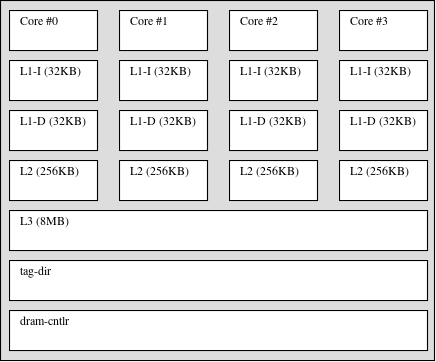
\includegraphics[width=0.5\textwidth]{output/npb-is/8way-lru/topo.png}
        %     \caption{Topology for \texttt{npb-is}, \texttt{splash2-ocean.cont}, and \texttt{splash2-radix} benchmark tests with all consistent cache sizes: 32 KB L1, 128 KS L2, and 512 KB L3. All benchmarks were run in \texttt{Sniper-7.3} with the \texttt{gainestown} configuration using the \texttt{--viz} and \texttt{--roi} options.}
        %     \label{topology} 
        % \end{figure}

    % \clearpage
    %%%%%%%%%%%%%%%%%%%%%%%%%%%%%%%%%%%%%%%%%%%%%%%%%%%%%%%%%%%%%%%%%%%%%%%%

    \section{Results \& Analysis}
    % \clearpage
    %%%%%%%%%%%%%%%%%%%%%%%%%%%%%%%%%%%%%%%%%%%%%%%%%%%%%%%%%%%%%%%%%%%%%%%%


    \section{Conclusion}
    \label{conclusion}
    % \clearpage
    %%%%%%%%%%%%%%%%%%%%%%%%%%%%%%%%%%%%%%%%%%%%%%%%%%%%%%%%%%%%%%%%%%%%%%%%

    \section{Appendix: Raw Post Processed Data}
    \label{appendix:raw}

    \subsection{benchmark} %%%%%%%%%%%%%%%%%%%%%%%%%%%%%%%%%%%
        
        \subsubsection{Power Results} %%%%%%%%%%%%%%%%%%%%%%%%%%%%%%%%%%%

        % Power
        % \begin{figure}[hbt!]
        %     \centering 
        %     \begin{adjustwidth}{-2.75cm}{}
        %     \begin{tabular}{ccc}
        %         \begin{subfigure}{0.42\textwidth}
        %             \centering
        %             \includegraphics[width=1\textwidth]{output/npb-is/8way-lru/power-chop.png}
        %             \caption{L3 energy 0.20 J; Total energy 16.79 J}
        %             \label{appfig:power:is:lru:8}
        %         \end{subfigure} &
        %         \begin{subfigure}{0.42\textwidth}
        %             \centering
        %             \includegraphics[width=1\textwidth]{output/npb-is/16way-lru/power-chop.png}
        %             \caption{L3 energy 0.21 J; Total energy 16.43 J}
        %             \label{appfig:power:is:lru:16}
        %         \end{subfigure} &
        %         \begin{subfigure}{0.42\textwidth}
        %             \centering
        %             \includegraphics[width=1\textwidth]{output/npb-is/32way-lru/power-chop.png}
        %             \caption{L3 energy 0.27 J; Total energy 16.40 J}
        %             \label{appfig:power:is:lru:32}
        %         \end{subfigure} 
        %     \end{tabular}
        %     \end{adjustwidth}
        %     \caption{Processor power with an (\ref{appfig:power:is:lru:8}) 8-way, (\ref{appfig:power:is:lru:16}) 16-way, and (\ref{appfig:power:is:lru:32}) 32-way L3 cache using LRU replacement policy.}
        %     \label{appfig:power:is:lru}
        % \end{figure}

        % legend
        % \begin{figure}
        %     \centering 
        %     \begin{adjustwidth}{-2.75cm}{}
        %     \begin{tabular}{ccc}
        %         & & 
        %         \begin{subfigure}{0.33\textwidth}
        %             \centering
        %             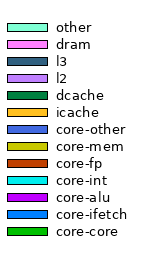
\includegraphics[width=1\textwidth]{output/npb-is/8way-lru/power-legend.png}
        %             % \caption{}
        %             \label{appfig:power:is:legend}
        %         \end{subfigure} 
        %     \end{tabular}
        % \end{adjustwidth}
        % \end{figure}
        % \clearpage

        % \begin{figure}[hbt!]
        %     \centering
        %     \noindent\begin{subfigure}{0.75\textwidth}
        %     \lstinputlisting{output/npb-is/8way-lru/power.out}
        %     \caption{}
        %     \end{subfigure}%

        %     \noindent\begin{subfigure}{0.75\textwidth}
        %     \lstinputlisting{output/npb-is/16way-lru/power.out}
        %     \caption{}
        %     \end{subfigure}%
        % \end{figure}
        % \clearpage

        % \begin{figure}[hbt!]\ContinuedFloat
        %     \centering
        %     \noindent\begin{subfigure}{0.75\textwidth}
        %     \lstinputlisting{output/npb-is/32way-lru/power.out}
        %     \caption{}
        %     \end{subfigure}%
        %     \caption{Specific values for each components' power consumption (See. Fig. \ref{appfig:power:is:lru}), for \texttt{npb-is} benchmark with (LRU) L3 associativity of (a) 8, (b) 16, and (c) 32 way.}
        %     \label{appfig:power:is:lru:values}
        % \end{figure}
        % \clearpage

        %%%%%%%%%%%%%%%%%%%%%%%%%%%%%%%%%%%%%%%%%%%%%%%%%%%%%%%%%%%%%%%%%%%%%%

        \subsubsection{CPI Stacks} %%%%%%%%%%%%%%%%%%%%%%%%%%%%%%%%%%%

        % CPI Result
        % \begin{figure}[hbt!]
        %     \centering 
        %     \begin{adjustwidth}{-2.75cm}{}
        %     \begin{tabular}{ccc}
        %         \begin{subfigure}{0.42\textwidth}
        %             \centering
        %             \includegraphics[width=1\textwidth]{output/npb-is/8way-lru/cpi-stack-chop.png}
        %             \caption{}
        %             \label{appfig:cpi:is:lru:8}
        %         \end{subfigure} &
        %         \begin{subfigure}{0.42\textwidth}
        %             \centering
        %             \includegraphics[width=1\textwidth]{output/npb-is/16way-lru/cpi-stack-chop.png}
        %             \caption{}
        %             \label{appfig:cpi:is:lru:16}
        %         \end{subfigure} &
        %         \begin{subfigure}{0.42\textwidth}
        %             \centering
        %             \includegraphics[width=1\textwidth]{output/npb-is/32way-lru/cpi-stack-chop.png}
        %             \caption{}
        %             \label{appfig:cpi:is:lru:32}
        %         \end{subfigure} 
        %     \end{tabular}
        %     \end{adjustwidth}
        %     \caption{CPI stack with an (\ref{appfig:cpi:is:lru:8}) 8-way, (\ref{appfig:cpi:is:lru:16}) 16-way, and (\ref{appfig:cpi:is:lru:32}) 32-way L3 cache using LRU replacement policy.}
        %     \label{appfig:cpi:is:lru}
        % \end{figure}

        % legend
        % \begin{figure}
        %     \centering 
        %     \begin{adjustwidth}{-2.75cm}{}
        %     \begin{tabular}{ccc}
        %         & 
        %         \begin{subfigure}{0.33\textwidth}
        %             \centering
        %             \includegraphics[width=1\textwidth]{output/npb-is/32way-rr/cpi-stack-legend.png}
        %             % \caption{}
        %             \label{appfig:cpi:is:legend1}
        %         \end{subfigure} 
        %         & 
        %         \begin{subfigure}{0.33\textwidth}
        %             \centering
        %             \includegraphics[width=1\textwidth]{output/npb-is/16way-srrip/cpi-stack-legend.png}
        %             % \caption{}
        %             \label{appfig:cpi:is:legend2}
        %         \end{subfigure} 
        %     \end{tabular}
        % \end{adjustwidth}
        % \end{figure}

        % Output Values
        % \begin{figure}[hbt!]
        %     \centering
        %     \noindent\begin{subfigure}{0.75\textwidth}
        %     \lstinputlisting{output/npb-is/8way-lru/cpi-stack.out}
        %     \caption{}
        %     \end{subfigure}%

        %     \noindent\begin{subfigure}{0.75\textwidth}
        %     \lstinputlisting{output/npb-is/16way-lru/cpi-stack.out}
        %     \caption{}
        %     \end{subfigure}%
        % % \end{figure}
        % % \clearpage

        % % \begin{figure}[hbt!]\ContinuedFloat
        % %     \centering
        %     \noindent\begin{subfigure}{0.75\textwidth}
        %     \lstinputlisting{output/npb-is/32way-lru/cpi-stack.out}
        %     \caption{}
        %     \end{subfigure}%
        %     \caption{Specific values for each components' CPI stack fraction of time (See. Fig. \ref{appfig:cpi:is:lru}), for \texttt{npb-is} benchmark with (LRU) L3 associativity of (a) 8, (b) 16, and (c) 32 way.}
        %     \label{appfig:cpi:is:lru:values}
        % \end{figure}
    % \clearpage
   %%%%%%%%%%%%%%%%%%%%%%%%%%%%%%%%%%%%%%%%%%%%%%%%%%%%%%%%%%%%%%%%%%%%%%

\end{document}